\documentclass[10pt]{article}
\usepackage[utf8]{inputenc}
\usepackage[T1]{fontenc}
\usepackage[margin=0.72in, top=0.68in, bottom=0.68in]{geometry}
\usepackage{times}
\usepackage{microtype}
\usepackage{amsmath,amssymb,amsfonts}
\usepackage{booktabs}
\usepackage{tabularx}
\usepackage{multirow}
\usepackage{enumitem}
\usepackage{xcolor}
\usepackage{hyperref}
\usepackage{tikz}
\usepackage{titlesec}
\usetikzlibrary{shapes.geometric, arrows.meta, positioning, fit, calc}

\hypersetup{
    colorlinks=true,
    linkcolor=blue!70!black,
    citecolor=blue!70!black,
    urlcolor=blue!70!black
}

\setlength{\parskip}{0.25em}
\setlength{\parindent}{0pt}
\setlist[itemize]{leftmargin=1.4em, itemsep=0.1em, topsep=0.12em}
\setlist[enumerate]{leftmargin=1.5em, itemsep=0.12em, topsep=0.12em}

\titlespacing*{\section}{0pt}{0.65em}{0.25em}
\titlespacing*{\subsection}{0pt}{0.45em}{0.18em}

\begin{document}

\begin{center}
    {\Large \textbf{Building a Plan-and-Verify Agent with Schema-Grounded Tool Retrieval and Policy Guardrails for VAKRA-Advanced (SemEval-2027 Task 11)}}\\[0.35em]
    {\normalsize \textbf{Team Member 1 Name} (\texttt{member1@email.edu}) \quad \& \quad \textbf{Team Member 2 Name} (\texttt{member2@email.edu})}\\
    {\small Advanced Natural Language Processing --- Course Project Proposal (Supervised by Prof.\ Nagwa El-Makky) \quad $|$ \quad November 19, 2026}
\end{center}
\vspace{-0.35cm}
\hrule
\vspace{0.15cm}

% ============================================================================
% SECTION 1: KEY INFORMATION
% ============================================================================
\section{Key Information}
\begin{itemize}
    \item \textbf{Project Title:} Building a Plan-and-Verify Agent with Schema-Grounded Tool Retrieval and Policy Guardrails for VAKRA-Advanced (SemEval-2027 Task 11)
    \item \textbf{Team Members:} [Team Member 1 Name] (\texttt{member1@email.edu}), [Team Member 2 Name] (\texttt{member2@email.edu})
    \item \textbf{Project Type \& Mentor:} Custom Shared-Task Project (\href{https://sites.google.com/view/vakrasemeval2027}{SemEval-2027 Task 11: VAKRA-Advanced}); Supervised by Prof.\ Nagwa El-Makky
    \item \textbf{Project Objective:} Design and build an autonomous tool-calling agent (\textbf{PV-VAKRA}) to solve the \textbf{two core VAKRA multi-hop reasoning tasks} (Task 1: Multi-Hop Structured API Reasoning [API Chaining, Tool Selection, and Multi-Hop Execution] and Task 2: Multi-Hop, Multi-Source Reasoning across APIs + Documents under Tool-Use Policies) and evaluate it on the official VAKRA benchmark.
\end{itemize}

% ============================================================================
% SECTION 2: RESEARCH PAPER SUMMARY (STRICTLY <= 2 PAGES: PAGES 1-2)
% ============================================================================
\section{Research Paper Summary (Baseline Agent \& Task Paper)}

\textbf{Bibliographical Information.}
\begin{itemize}
    \item \textbf{Title:} \textit{VAKRA: Evaluating Multi-Hop Reasoning Across APIs and Retrieval Under Tool-Use Policies}
    \item \textbf{Authors:} Ankita Rajaram Naik, Anupama Narasimha Murthi, Benjamin T. Elder, Siyu Huo, Praveen Venkateswaran, Abdulhamid Adebayo, Sara Rosenthal, and Danish Contractor (IBM Research)
    \item \textbf{Venue \& Year:} arXiv Preprint (\texttt{arXiv:2608.12282}), 2026 (Official Baseline Agent \& Evaluation Framework for SemEval-2027 Task 11)
    \item \textbf{URLs:} \url{https://arxiv.org/abs/2608.12282} \ $|$ \ Baseline Agent Code: \url{https://github.com/IBM/vakra} \ $|$ \ Data: \url{https://huggingface.co/datasets/ibm-research/VAKRA}
\end{itemize}

\textbf{Background and Motivation.}
Autonomous Large Language Model (LLM) agents deployed in enterprise workflows must solve two intertwined reasoning problems: (1) \textbf{Multi-Hop Structured API Reasoning}, where an agent selects relevant tools from thousands of candidate APIs and chains $3\text{--}7$ dependent function calls by passing intermediate JSON outputs as downstream parameters, and (2) \textbf{Multi-Hop, Multi-Source Reasoning under Tool-Use Policies}, where the agent dynamically combines structured API executions with unstructured document retrieval (RAG) while obeying strict natural-language organizational policies (e.g., data privacy or source-authority constraints). Existing agent architectures such as standard \textbf{ReAct} \cite{yao2023react} interleave single-step reasoning and tool execution greedily. Naik et al.\ \cite{naik2026vakra} formalize these two multi-hop tasks in a realistic executable environment ($8,000+$ Python APIs across $62$ domains) and implement a standardized ReAct baseline agent to diagnose why current LLM agents fail on long-horizon, policy-constrained workflows.

\textbf{Summary of Contributions.}
From an agent-modeling and evaluation perspective, Naik et al.\ \cite{naik2026vakra} make three central contributions:
\begin{enumerate}
    \item \textbf{Formulation of Two Core Multi-Hop Agent Tasks (Spanning Four Subtasks):} Given a user query $q$, natural-language tool-use policy $\mathcal{P}$, candidate API library $\mathcal{T}$, and unstructured document corpus $\mathcal{D}$, the agent must synthesize an execution trajectory $\tau = \langle (t_1, a_1, o_1), \dots, (t_K, a_K, o_K), \hat{y} \rangle$, where $t_k \in \mathcal{T} \cup \{\textsc{Retrieve}\}$ is the invoked tool, $a_k$ is its argument dictionary, $o_k = \text{Exec}(t_k, a_k)$ is the live execution output, and $\hat{y}$ is the grounded final response. This formulation encompasses \textbf{Task 1: Multi-Hop Structured API Reasoning} (covering Subtask 1: API Chaining over compositional Business Intelligence APIs, Subtask 2: Tool Selection from $150+$ APIs per slice, and Subtask 3: $3\text{--}7$ hop API reasoning) and \textbf{Task 2: Multi-Hop, Multi-Source Reasoning} (Subtask 4: integrating API calls and document RAG across $664$ queries, including $244$ policy-constrained queries).
    \item \textbf{Standardized ReAct Baseline Agent \& Deterministic Trajectory Evaluator:} The authors implement a unified ReAct agent harness that conditions the LLM on $(q, \mathcal{P}, \mathcal{T}_{\text{slice}})$ to iteratively generate $\text{Thought}_k \rightarrow \text{Action}(t_k, a_k) \rightarrow \text{Observation}(o_k)$. Because multiple API sequences can validly solve a query, the agent's predicted trajectory $\tau$ is evaluated by re-executing calls against live databases and verifying state equivalence and policy compliance:
    \begin{equation}
        \text{Score}(\tau, q, \mathcal{P}) = \mathbb{I}\!\left[\text{ExecState}(\tau) \equiv \text{ExecState}(\tau^*)\right] \cdot \mathbb{I}\!\left[\forall k \in \{1..K\},\ (t_k, a_k) \models \mathcal{P}\right] \cdot \text{Acc}(\hat{y}, y^*)
    \end{equation}
    \item \textbf{Empirical Diagnosis of ReAct Agent Bottlenecks:} Benchmarking frontier and open-weight LLMs within the ReAct baseline reveals severe architectural weaknesses: while the baseline agent achieves up to \textbf{70.4\%} accuracy on 1-hop query-aligned APIs, accuracy drops to \textbf{50\%--51\%} on compositional BI API chaining, degrades by \textbf{$>$50\%} across $3\text{--}7$ reasoning hops, and collapses to \textbf{2.4\%} on policy-constrained unanswerable queries. Crucially, trace-level error analysis proves that failures are rarely JSON syntax errors; rather, the ReAct agent fails due to \textit{cross-source entity disambiguation errors}, \textit{intermediate schema misalignments}, and \textit{policy instruction-forgetting}.
\end{enumerate}

\textbf{Limitations of the Baseline Agent and Critical Discussion.}
Critically examining the baseline agent in Naik et al.\ \cite{naik2026vakra} exposes three architectural flaws that directly motivate our proposed agent:
\begin{itemize}
    \item \textbf{Myopic Greedy Execution Without Lookahead or Backtracking:} The baseline ReAct agent selects one tool at a time without constructing a global dependency plan. If hop $k=1$ invokes an endpoint whose output schema lacks the foreign key required at hop $k=2$, the agent has no explicit backtracking or schema-compatibility lookahead to recover.
    \item \textbf{Lack of Explicit Cross-Source Entity Grounding Memory:} When transitioning from an unstructured document hop ($\textsc{Retrieve}$) to a structured database API hop, the baseline agent stuffs raw text chunks into the prompt history. It frequently passes unnormalized surface strings (e.g., ``Big Blue'') into strict SQL-backed API parameters expecting canonical IDs (\texttt{company\_id="IBM\_01"}).
    \item \textbf{Passive Prompt-Only Policy Conditioning:} The baseline agent simply appends policy $\mathcal{P}$ to the system prompt. As multi-hop JSON observations accumulate ($>8\text{k}$ tokens), attention dilution causes the LLM to ignore policy restrictions, explaining the $97.6\%$ failure rate on unanswerable policy-constrained queries.
\end{itemize}
Despite these limitations of its baseline agent, the paper is highly convincing: its trace-level diagnosis clearly isolates the exact reasoning bottlenecks that a superior agent architecture must overcome.

\textbf{Why This Paper?}
We selected Naik et al.\ \cite{naik2026vakra} because it defines the exact problem formulation, evaluation metrics, and official \textbf{ReAct Baseline Agent} for \textbf{SemEval-2027 Task 11 (VAKRA-Advanced)}. Analyzing the paper's failure taxonomy gave us the blueprint for our own agent design: to beat the VAKRA baseline, we must replace greedy ReAct with a \textit{Plan-and-Verify Agent} featuring schema-graph retrieval, structured entity-linking memory, and an active pre-execution policy verifier.

\textbf{Wider Research Context.}
In the broader landscape of NLP and Deep Learning, building agents for multi-hop, multi-source tool use advances \textit{neuro-symbolic program synthesis} and \textit{grounded compositional reasoning}. Rather than treating language models as static text generators, tool-augmented agent architectures use natural language as a control interface to orchestrate symbolic computation (SQL/Python APIs) alongside unstructured reading comprehension (RAG), a paradigm central to reliable enterprise AI.

\newpage
% ============================================================================
% SECTION 3: CONCISE SOTA SURVEY (STRICTLY <= 2 PAGES: PAGES 3-4)
% ============================================================================
\section{Concise SOTA Survey of Tool-Calling Agent Architectures}

Because our project focuses on \textbf{building an agent to solve multi-hop structured API and multi-source reasoning tasks} (and evaluating it on the VAKRA benchmark), we survey \textbf{six recent state-of-the-art agent architectures and tool-retrieval methods (2023--2026)}.

\subsection{Review of Recent Agent Architectures and Tool-Use Methods}

\textbf{1. VAKRA Baseline ReAct Agent (Naik et al., 2026 \cite{naik2026vakra}; Yao et al., ICLR 2023 \cite{yao2023react}).}
The official VAKRA baseline employs the \textbf{ReAct} (\textit{Reasoning + Acting}) architecture paired with dense retrieval over tools and documents. At each step $k$, the LLM generates a free-form reasoning trace ($\text{Thought}_k$) conditioned on previous observations, emits a single tool call $(t_k, a_k)$, and appends the raw output $o_k$ to its context window. While effective on 1-hop calls ($70.4\%$), its greedy single-path execution and passive system-prompt policy conditioning cause $>50\%$ degradation over $3\text{--}7$ hops and $2.4\%$ accuracy on unanswerable policy queries.

\textbf{2. ToolLLM: Neural API Retriever + DFSDT Agent (Qin et al., ICLR 2024) \cite{qin2024toolllm}.}
To scale tool-calling agents to thousands of APIs, ToolLLM introduces a two-stage agent architecture: (i) a contrastive dense \textit{Neural API Retriever} that encodes user instructions and API documentation to retrieve top-$K$ candidate tools, and (ii) a \textit{Depth-First Search-based Decision Tree (DFSDT)} agent controller. Unlike greedy ReAct, DFSDT allows the agent to expand multiple action branches and explicitly backtrack when an API call returns an error or empty payload.

\textbf{3. AnyTool: Hierarchical Retrieval + Self-Reflective Agent (Du et al., ICML 2024) \cite{du2024anytool}.}
AnyTool addresses two failure modes of ToolLLM: flat dense retrieval struggles to disambiguate fine-grained endpoints across large API pools, and open-loop DFSDT often terminates before fully answering multi-part queries. AnyTool designs a \textit{three-tier Hierarchical Retriever Agent} (Meta-Agent $\rightarrow$ Category Agents $\rightarrow$ Tool-Pool Manager) combined with a \textit{Self-Reflective Solver} that verifies whether the candidate output satisfies the user query and re-invokes retrieval/search with refined queries if verification fails.

\textbf{4. ReWOO: Decoupled Plan-then-Execute Agent (Xu et al., 2023/2024) \cite{xu2023rewoo}.}
ReWOO (\textit{Reasoning Without Observation}) replaces ReAct's step-by-step interleaved loop with a modular three-module architecture: (\textit{Planner} $\rightarrow$ \textit{Worker} $\rightarrow$ \textit{Solver}). The \textit{Planner} constructs a complete multi-step dependency DAG upfront using symbolic variable placeholders (e.g., $\texttt{\#E1} = \text{Tool}_1(q)$, $\texttt{\#E2} = \text{Tool}_2(\texttt{\#E1})$); the \textit{Worker} executes the bound API calls; and the \textit{Solver} synthesizes the final response. This decoupled planning reduces token consumption by $5\times$ and prevents mid-trajectory distraction from verbose JSON payloads.

\textbf{5. LATS: Language Agent Tree Search (Zhou et al., ICML 2024) \cite{zhou2024lats}.}
LATS unifies planning, acting, and reflection by framing tool-augmented LLM reasoning as \textit{Monte Carlo Tree Search (MCTS)}. It uses the LLM both as a policy proposer and as an evaluator assigning scalar value scores $V(s_k)$ to intermediate execution states, backed by verbal self-reflection when trajectories fail. While highly accurate on complex multi-hop reasoning, full MCTS incurs substantial LLM call and latency overhead.

\textbf{6. Re-Invoke (Chen et al., EMNLP 2024) \cite{chen2024reinvoke} \& Gorilla (Patil et al., NeurIPS 2024) \cite{patil2024gorilla}.}
Gorilla trains retriever-aware LLMs to reduce parameter hallucination when conditioned on retrieved API documentation. Complementing Gorilla, \textit{Re-Invoke} improves zero-shot tool selection for multi-hop queries via two mechanisms: offline \textit{Document-to-Query Generation} (enriching each API's index representation with synthetic user intents) and online \textit{Multi-Intent Query Rewriting} (decomposing complex prompts into sub-queries before dense ranking).

\subsection{Comparative Analysis of SOTA Agent Methods, Datasets, and Limitations}

Table \ref{tab:sota_comparison} compares these six agent methods across architecture design, evaluation benchmarks, and unresolved limitations when applied to VAKRA-Advanced's two core tasks.

\begin{table}[!htbp]
\centering
\footnotesize
\renewcommand{\arraystretch}{1.12}
\begin{tabularx}{\textwidth}{>{\raggedright\arraybackslash}p{2.2cm} >{\raggedright\arraybackslash}p{3.4cm} >{\raggedright\arraybackslash}p{2.6cm} >{\raggedright\arraybackslash}p{2.2cm} >{\raggedright\arraybackslash}X}
\toprule
\textbf{Agent / Method} & \textbf{Agent Architecture \& Technique} & \textbf{Evaluated Datasets} & \textbf{Key Metrics} & \textbf{Limitations on Multi-Hop \& Multi-Source Tasks} \\
\midrule
\textbf{ReAct Baseline} \cite{yao2023react,naik2026vakra} & Greedy interleaved Thought $\rightarrow$ Action $\rightarrow$ Observation + prompt policy & \textbf{VAKRA} ($8,000+$ APIs, $62$ domains, $664$ multi-source queries) & Trace Replay \texttt{Exec-Acc}, Answer Acc. & Myopic 1-step horizon ($>50\%$ drop on $3\text{--}7$ hops); prompt-only policy fails ($2.4\%$ on unanswerable queries). \\
\midrule
\textbf{ToolLLM (DFSDT)} \cite{qin2024toolllm} (ICLR 2024) & Contrastive Dense API Retriever + Depth-First Search Decision Tree & \textbf{ToolBench} ($16,464$ REST APIs), APIBench & Pass Rate \& Win Rate & Flat retriever misses intermediate bridge APIs; lacks cross-source entity linking between RAG text and SQL APIs. \\
\midrule
\textbf{AnyTool} \cite{du2024anytool} (ICML 2024) & 3-Tier Hierarchical Retriever Agent + Self-Reflective DFSDT Solver & \textbf{AnyToolBench} \& ToolBench ($16\text{k}+$ APIs) & Rubrics Pass Rate, Recall@$K$ & High multi-agent token cost; self-reflection checks final answer completeness but not strict tool-use policies. \\
\midrule
\textbf{ReWOO} \cite{xu2023rewoo} (2023/2024) & Decoupled Planner (symbolic DAG \texttt{\#E1}$\rightarrow$\texttt{\#E2}) + Worker + Solver & HotpotQA, TriviaQA, Tool QA benchmarks & Exact Match, F1, Token Efficiency & Open-loop static plan breaks if an intermediate RAG/API output requires dynamic entity disambiguation or fallback. \\
\midrule
\textbf{LATS} \cite{zhou2024lats} (ICML 2024) & Monte Carlo Tree Search (MCTS) + LLM Value Function + Verbal Reflection & HotpotQA, WebShop, Programming tasks & Success Rate, Exact Match & Prohibitive inference latency ($10\text{--}30\times$ rollouts per query); does not model API I/O schema graphs. \\
\midrule
\textbf{Re-Invoke} \cite{chen2024reinvoke} \& \textbf{Gorilla} \cite{patil2024gorilla} & Synthetic query-enriched indexing + Multi-intent query decomposition & ToolBench, ToolE, APIBench ($1.6\text{k}\text{--}16\text{k}$ APIs) & Recall@$K$, NDCF, AST Match & Retrieves tools matching explicit user sub-queries, missing implicit bridge APIs whose schemas link hop $k$ to hop $k+1$. \\
\bottomrule
\end{tabularx}
\vspace{-0.15cm}
\caption{Comparison of SOTA agent architectures and tool-retrieval methods relevant to solving VAKRA-Advanced.}
\label{tab:sota_comparison}
\vspace{-0.15cm}
\end{table}

\textbf{Synthesis of Architectural Gaps Our Agent Solves.}
Comparing the methods in Table \ref{tab:sota_comparison} reveals why existing agents struggle on VAKRA's two core tasks:
(1) \textbf{Bridge Tool Discovery:} Query-decomposition retrievers (\textit{Re-Invoke}, \textit{AnyTool}) only retrieve tools semantically similar to the prompt $q$, missing intermediate bridge APIs $t_2$ in chains $t_1 \rightarrow t_2 \rightarrow t_3$ that can only be identified via \textit{input-output schema compatibility}.
(2) \textbf{Adaptive DAG Planning with Cross-Source Entity Grounding:} \textit{ReWOO}'s decoupled DAG planning avoids ReAct's context bloat, but static open-loop plans fail when unstructured RAG entities must be dynamically resolved into canonical SQL database IDs.
(3) \textbf{Pre-Execution Policy Guardrails:} Neither \textit{DFSDT}, \textit{AnyTool}, nor \textit{LATS} enforces natural-language tool-use constraints before tool invocation. Our proposed \textbf{PV-VAKRA} agent unifies schema-graph retrieval, adaptive DAG planning with an entity scratchpad, and pre-execution policy verification.

\clearpage
% ============================================================================
% SECTION 4: PROJECT DESCRIPTION (STRICTLY <= 2 PAGES: PAGES 5-6)
% ============================================================================
\section{Project Description}

\subsection{Main Goals and Scientific Question}
Our goal is to design and build an autonomous agent, \textbf{PV-VAKRA} (\textit{Plan-and-Verify Agent}), to solve the two core multi-hop reasoning tasks in \textbf{SemEval-2027 Task 11 (VAKRA-Advanced)} and evaluate it on the official VAKRA benchmark. We address the following scientific question:
\begin{quote}
\vspace{-0.15cm}
\textit{Can an agent architecture that integrates (1) Schema-Graph-Guided Tool Retrieval, (2) Adaptive DAG Planning with an Explicit Cross-Source Entity Scratchpad, and (3) Pre/Post-Execution Policy Guardrail Verification significantly outperform the official VAKRA ReAct baseline agent across both Multi-Hop Structured API Reasoning (Task 1) and Policy-Constrained Multi-Hop Multi-Source Reasoning (Task 2)?}
\vspace{-0.15cm}
\end{quote}
\textbf{Motivation \& Stretch Goals:} Rather than relying on greedy ReAct loops or expensive MCTS rollouts, our agent directly targets the three empirical failure modes identified on the VAKRA benchmark: bridge-tool retrieval misses, cross-source RAG-to-SQL entity mismatches, and policy violations. As stretch goals, we will (i) fine-tune a compact open-weight agent (\texttt{Qwen2.5-7B-Instruct}) via Direct Preference Optimization (DPO) on verified vs.\ policy-violating trajectories generated by our pipeline, and (ii) submit our agent's predictions to the official SemEval-2027 Task 11 leaderboard.

\subsection{NLP Tasks Addressed by Our Agent}
Our agent solves the \textbf{two core problem settings of VAKRA} (which span all four subtasks of SemEval-2027 Task 11 \cite{naik2027semeval}):
\begin{itemize}
    \item \textbf{Task 1 --- Multi-Hop Structured API Reasoning (Subtasks 1, 2, \& 3):} Given a user query $q$ and a candidate pool of $150+$ domain APIs (drawn from $8,000+$ total APIs), the agent must select the exact required tools (\textit{Subtask 2: Tool Selection}), compose sequential or nested calls (\textit{Subtask 1: API Chaining}), and execute $3\text{--}7$ dependent hops where JSON fields returned at hop $k$ parameterize hop $k+1$ (\textit{Subtask 3: Multi-Hop API Reasoning}).
    \item \textbf{Task 2 --- Multi-Hop, Multi-Source Reasoning under Policies (Subtask 4):} Given query $q$ and a natural-language tool-use policy $\mathcal{P}$, the agent must interleave structured API calls with unstructured document retrieval ($\textsc{Retrieve}(q_{\text{doc}}, \mathcal{D})$), resolve entities across sources, and strictly obey policy $\mathcal{P}$ (including abstaining when $\mathcal{P}$ prohibits the required data source).
\end{itemize}
\textbf{Concrete Input/Output Example Solved by Our Agent:}
\textit{Input Query $q$:} ``What is the total Q3 reimbursement approved for the lead auditor named in the 2025 Compliance Memo, and what is their department's remaining budget?'' \textit{Policy $\mathcal{P}$:} ``Do not query personal payroll endpoints; if reimbursement data requires restricted HR-Payroll APIs, abstain and cite the policy violation.''
\textit{Agent Trajectory $\tau$:} Hop 1: Retrieve ``2025 Compliance Memo'' $\rightarrow$ extracts \texttt{"Dr.\ E.\ Vance"}. Hop 2: Call \texttt{get\_employee("E. Vance")} $\rightarrow$ resolves \texttt{emp\_id="E409"}, \texttt{dept\_id="D12"} in the Entity Scratchpad. Hop 3: Policy Verifier blocks restricted \texttt{get\_payroll\_reimbursement("E409")} per $\mathcal{P}$, permits \texttt{get\_dept\_budget("D12")}.
\textit{Agent Output $\hat{y}$:} Reports Department D12's remaining budget while abstaining from the restricted HR-Payroll reimbursement query per Policy $\mathcal{P}$.

\subsection{Evaluation Benchmark Dataset and Preprocessing}
We will train, develop, and evaluate our agent on the official \textbf{VAKRA benchmark} (\texttt{ibm-research/VAKRA} on Hugging Face and \texttt{IBM/vakra} on GitHub) \cite{naik2026vakra}. The benchmark provides $8,000+$ locally executable Python APIs across $62$ enterprise domains backed by SQLite databases and aligned document collections, including single-hop/compositional BI splits, multi-hop structured API splits ($2\text{--}7$ hops), and the $664$-sample Multi-Hop Multi-Source split ($420$ unconstrained + $244$ policy-constrained queries).
\textbf{Agent Offline Indexing \& Preprocessing:}
(1) \textit{API Input-Output Compatibility Graph Construction:} Our agent parses all $8,000+$ Python function docstrings, argument types, and return schemas offline to build a directed \textbf{Schema Compatibility Graph} $\mathcal{G} = (\mathcal{T}, \mathcal{E})$, adding directed edge $(t_i \rightarrow t_j) \in \mathcal{E}$ whenever an output field of $t_i$ matches the semantic type or foreign-key signature of an input parameter of $t_j$.
(2) \textit{Hybrid Tool \& Document Indexing:} We index API schemas (enriched with synthetic user intents following Re-Invoke \cite{chen2024reinvoke}) and document chunks using BM25 + dense embeddings (\texttt{BAAI/bge-large-en-v1.5}).

\subsection{Proposed Agent Architecture and Neural Methods}
Figure \ref{fig:arch} illustrates our four-stage \textbf{PV-VAKRA} agent architecture:

\begin{figure}[h!]
\centering
\vspace{-0.1cm}
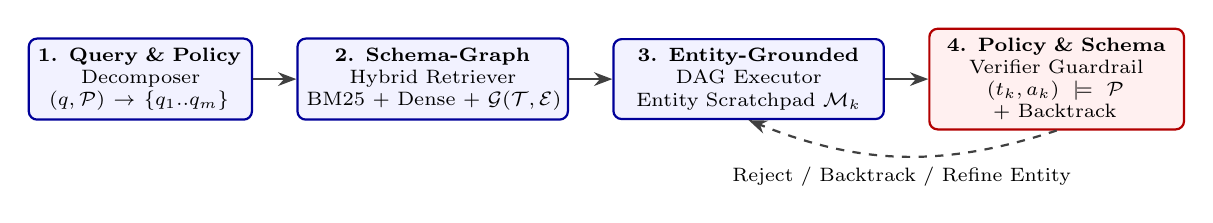
\begin{tikzpicture}[
    node distance=0.45cm and 0.55cm,
    box/.style={rectangle, rounded corners=3pt, draw=blue!60!black, fill=blue!5, thick, minimum height=0.95cm, align=center, font=\scriptsize},
    guard/.style={rectangle, rounded corners=3pt, draw=red!70!black, fill=red!6, thick, minimum height=0.95cm, align=center, font=\scriptsize},
    arrow/.style={-Stealth, thick, draw=black!75}
]
\node[box, text width=2.6cm] (q) {\textbf{1. Query \& Policy}\\Decomposer\\$(q, \mathcal{P}) \rightarrow \{q_1..q_m\}$};
\node[box, text width=3.2cm, right=of q] (ret) {\textbf{2. Schema-Graph}\\Hybrid Retriever\\BM25 + Dense + $\mathcal{G}(\mathcal{T},\mathcal{E})$};
\node[box, text width=3.2cm, right=of ret] (plan) {\textbf{3. Entity-Grounded}\\DAG Executor\\Entity Scratchpad $\mathcal{M}_k$};
\node[guard, text width=3.0cm, right=of plan] (pol) {\textbf{4. Policy \& Schema}\\Verifier Guardrail\\$(t_k, a_k) \models \mathcal{P}$ + Backtrack};

\draw[arrow] (q) -- (ret);
\draw[arrow] (ret) -- (plan);
\draw[arrow] (plan) -- (pol);
\draw[arrow, dashed, bend left=20] (pol.south) to node[below, font=\scriptsize] {Reject / Backtrack / Refine Entity} (plan.south);
\end{tikzpicture}
\vspace{-0.25cm}
\caption{Architecture of our proposed \textbf{PV-VAKRA} Agent for solving Tasks 1 \& 2 on the VAKRA benchmark.}
\label{fig:arch}
\vspace{-0.15cm}
\end{figure}

\begin{enumerate}
    \item \textbf{Intent Decomposer \& Schema-Graph Hybrid Tool Retriever (Solves Tool Selection \& Chaining):} Following Re-Invoke \cite{chen2024reinvoke}, our agent decomposes query $q$ into atomic sub-goals $\{q_1, \dots, q_m\}$ and retrieves initial candidate APIs via $s_{\text{ret}}(q_i, t) = \lambda\,\text{cos}(\mathbf{e}(q_i), \mathbf{e}(t)) + (1-\lambda)\,\text{BM25}(q_i, t)$. Crucially, to discover intermediate bridge APIs missed by query similarity, we expand the top-$k_0$ retrieved tools with their $1$-hop neighbors on the \textbf{Schema Compatibility Graph} $\mathcal{G}(\mathcal{T}, \mathcal{E})$ and rerank candidates with a cross-encoder (\texttt{bge-reranker-v2-m3}).
    \item \textbf{Adaptive DAG Planner \& Cross-Source Entity Scratchpad (Solves Multi-Hop \& Multi-Source Grounding):} Inspired by ReWOO \cite{xu2023rewoo}, the planner constructs a symbolic execution DAG over the retrieved tools. To prevent cross-source grounding failures, the executor maintains a structured key-value \textbf{Entity Scratchpad} $\mathcal{M}_k$ storing tuples of $(\text{mention}, \text{id}, \text{source}, \text{type})$. Whenever an unstructured RAG passage yields a named entity, an \textit{Entity Resolution Sub-step} invokes lookup APIs to map the surface mention to a canonical database key before executing downstream analytical APIs.
    \item \textbf{Stepwise Schema \& Policy Guardrail Verifier (Solves Policy Adherence \& Error Recovery):} Before executing any proposed tool call $(t_k, a_k)$ and before emitting $\hat{y}$, our \textbf{Policy Verifier} parses policy $\mathcal{P}$ into atomic rules $\{c_1, \dots, c_L\}$ and evaluates entailment $P_{\text{verify}}(\mathcal{P} \models \neg(t_k, a_k))$. If a policy violation or empty/invalid schema output is detected, the verifier blocks execution and triggers local DFSDT-style backtracking (up to $B=2$ retries) or safe policy-compliant abstention.
\end{enumerate}
\textbf{Downloaded vs.\ Original Implementation:} We download the official \texttt{IBM/vakra} benchmark environment/evaluator, pretrained open-weight LLMs (\texttt{Qwen2.5-14B/32B}, \texttt{Llama-3.3-70B}), and pretrained retriever checkpoints (\texttt{bge-large-en-v1.5} and \texttt{bge-reranker-v2-m3}). \textbf{We implement from scratch as our original agent contributions:} (1) the Schema Compatibility Graph builder $\mathcal{G}(\mathcal{T}, \mathcal{E})$ and graph-expanded bridge retriever, (2) the Adaptive DAG Controller with the Cross-Source Entity Scratchpad $\mathcal{M}_k$, and (3) the Pre/Post-Execution Policy Guardrail Verifier.

\subsection{Baselines and Quantitative/Qualitative Evaluation on the VAKRA Benchmark}
\textbf{Baselines:} We will evaluate our \textbf{PV-VAKRA} agent against: (1) the official \texttt{IBM/vakra} \textbf{ReAct Baseline Agent} run locally on identical backbone LLMs + published scores in Naik et al.\ \cite{naik2026vakra}; (2) a \textbf{Flat Dense Retrieval + ReAct Agent} without $\mathcal{G}(\mathcal{T}, \mathcal{E})$; and (3) \textbf{Ablated Agents} (removing the Policy Verifier or Entity Scratchpad).
\textbf{Quantitative Metrics on VAKRA:} Using the official VAKRA evaluation suite, we measure: (1) \textbf{Trajectory Execution Accuracy (Exec-Acc)} via live database/RAG replay, (2) \textbf{Final Answer Accuracy / Token F1}, (3) \textbf{Tool Selection Recall@$K$ \& F1}, and (4) \textbf{Policy Compliance \& Abstention F1}. We compare directly against VAKRA's published ReAct baseline scores (\textbf{70.4\%} single-hop, \textbf{50\%--51\%} compositional BI, \textbf{$>$50\%} multi-hop drop, and \textbf{2.4\%} on unanswerable policy-constrained queries), alongside qualitative error stratification across hop depths ($2\text{--}7$ hops).

\subsection{Ethical Challenges, Societal Risks, and Mitigation Strategies}
Deploying autonomous tool-calling agents over enterprise databases and document stores poses at least two significant ethical and societal risks. First, \textbf{unauthorized tool execution and policy bypass}: in enterprise deployments, an agent that fails to respect natural-language compliance rules (as shown by the $97.6\%$ failure rate on unanswerable policy queries in baseline VAKRA models) could invoke restricted endpoints, expose confidential employee or customer PII, or trigger unauthorized state-mutating financial transactions. Second, \textbf{compounded cross-source hallucination in high-stakes decisions}: when an agent mislinks an ambiguous entity between an unstructured memo and a structured database across a 5-hop chain, it outputs a fabricated figure with a false veneer of API-backed authority, risking harmful decisions in healthcare, legal, or financial auditing. To mitigate these risks, we incorporate three concrete safeguards into our agent: (1) a \textbf{strict pre-execution Policy Guardrail Verifier} that defaults to safe abstention whenever policy entailment confidence falls below a calibrated threshold $\tau_{\text{safe}}$, (2) restricting execution to \textbf{sandboxed, read-only database transactions} unless explicit human-in-the-loop authorization is granted for state-mutating APIs, and (3) emitting \textbf{verifiable provenance traces} linking every claim in the final answer to its exact API payload or document span.

{\footnotesize
\bibliographystyle{plain}
\bibliography{references}
}

\end{document}
